\documentclass[a4paper,12pt]{article}
\title{Análisis Rodrigo}
\author{D\'ebora Chan}
\date{}
\usepackage{color,colortbl, soul}
\usepackage{fancybox}
\input{xy}
\xyoption{all}
\xyoption{poly}
\usepackage[all]{xy}
\usepackage[dvipsnames]{xcolor}
\usepackage{tcolorbox}
\usepackage[spanish,es-tabla]{babel}
\usepackage{dcolumn}
\usepackage{slashbox}
\usepackage{colortbl}
\usepackage{rotating}
\usepackage{longtable}
\usepackage {bezier}
\usepackage[utf8]{inputenc}
\usepackage{amsmath,amsthm,amsfonts,amssymb,stmaryrd}
\usepackage{latexsym}
\usepackage{a4,color,palatino,fancyhdr,fancybox,colortbl}
\usepackage{booktabs,tabularx,tabulary,tabularht,tabularkv}
\usepackage{framed,tikz,pgf,fancybox}
\usetikzlibrary{positioning,shapes,shadows,arrows}
\usepackage{pdfpages} 
\usepackage{siunitx}
\usepackage{multirow,array, float, tabularx}
\usepackage{graphicx} % figuras
\usepackage{subfigure} % subfiguras
\usepackage{graphicx}%poner [dvips] para gráficos
\usepackage{float}%Este packete permite controlar la flotacion de figuras al poner [H] o [h] como opcion de \begin{figure}
\usepackage [spanish]{babel}
\usepackage[small, bf, margin=90pt, tableposition=bottom]{caption}
\renewcommand{\baselinestretch}{1.5}
\RequirePackage{amssymb}
\RequirePackage[T1]{fontenc}
\newtheorem{teo}{Teorema}


\newtheorem{theorem}{Teorema}
\newtheorem{obs}[theorem]{Observación}
\newtheorem{coro}[theorem]{Corolario}
\newtheorem{claim}[theorem]{Claim}
\newtheorem{conclusion}[theorem]{Conclusi\'{o}n}
\newtheorem{definition}[theorem]{Definici\'{o}n}
\newtheorem{ejemplo}[theorem]{Ejemplo}
\newtheorem{exercise}[theorem]{Ejercicio}
\newtheorem{lemma}[theorem]{Lema}
\newtheorem{proposition}[theorem]{Proposici\'{o}n}
\newtheorem{prop}[theorem]{Propiedad}
\newtheorem{remark}[theorem]{Observaci?n}
\newtheorem{solution}[theorem]{Soluci\'{o}n}
\newtheorem{summary}[theorem]{Summary}

\begin{document}
\section{Análisis de la varianza}

\begin{center}
	\fcolorbox{purple}{cyan!10}{¿Por qué el análisis de la varianza para comparar varios grupos?
	}
\end{center}


Si hacemos la comparación de a pares, es decir si tenemos $k$ grupos, deberíamos realizar $k(k-1)/2$ contrastes. Considerando un nivel de significación $\alpha$, la probabilidad de no cometer error de tipo I en todos ellos, es decir el nivel de significación global es: $1-(1-\alpha)^{k(k-1)/2}$.

Por ejemplo, si el nivel de significación para cada comparación se estableciera  en el  $0.05$ y la cantidad de grupos fuera $k=5$  el número de comparaciones es 10 y el nivel de signficación global sería del $$1-(1-0.05)^{10} = 0.4012$$

Es decir que:
\textcolor{BlueGreen}{\textsc{ La probabilidad de cometer algún error crece notablemente!!!}}

Una mejor respuesta para este problema, desarrollada por Fisher, es comparar las medias de tres o más poblaciones independientes con distribuciones normales de igual varianza. El análisis que corresponde es el que desarrollaremos a continuación y se denomina análisis de la varianza (ADEVA) o en inglés analysis of variance (ANOVA).

Disponemos de $k$ muestras 
	normales independientes con varianzas iguales, con $n_i$ observaciones en cada una de ellas.
	
	Muestra 1: \textcolor{BlueGreen}{ $$ X_{11}, X_{12},…, X_{1n_1} \hspace{0.3cm} \text{ v.a.i.i.d.}      \hspace{0.3cm} X_{1i}\sim  N(\mu_1, \sigma^2)$$}
	….......….................................................................\\
	Muestra i:   \textcolor{BlueGreen}{ $$ X_{i1}, X_{i2},…, X_{in_i}\hspace{0.3cm} \text{ v.a.i.i.d.}      \hspace{0.3cm} X_{ij}\sim  N(\mu_i, \sigma^2)$$}
	….......…......................................................................\\
	Muestra k:  \textcolor{BlueGreen}{$$ X_{k1}, X_{k2},…, X_{kn_k}\hspace{0.3cm} \text{ v.a.i.i.d.}      \hspace{0.3cm} X_{ki}\sim  N(\mu_k, \sigma^2)$$}




\textbf{\textcolor{BlueGreen}{Modelo}}

\[X_{ij}=\mu+\alpha_i+\epsilon_{ij} , \text{con} 1 \leq i \leq k, 1 \leq j \leq n_i
\]
siendo
\[
\epsilon_{ij}\sim N(0,\sigma^2) \hspace{0.3cm} \text{independientes}
\]
\[
\alpha_i \text{se conoce como el efecto del grupo i-simo} 
\]
\begin{center}
	\fbox{\parbox[t][2.4cm][b]{15cm}{	\textbf{\textcolor{BlueGreen!70}{Las variables aleatorias observadas  son normales, independientes entre sí dentro de las muestras y entre las muestras y homocedásticas (con varianzas iguales).}}}}
\end{center}

Estos son los supuestos del modelo en los que se basan los intervalos y test que se construyen a partir de ellos. Es decir que si no se cumplen los supuestos del modelo, los test podrían no cumplirse.

\textcolor{BlueGreen}{Idea de Fisher}
La idea de Fisher es comparar las estimaciones de la varianza $\sigma$ común a los k grupos realizadas suponiendo que las medias son iguales y sin suponerlo.

Si las estimaciones son similares implica que las medias no son diferentes, en cambio si las estimaciones son distintas implica que las medias lo son.

Una de las estimaciones es estimando la varianza en cada grupo y luego amalgamando entre los grupos. Se la suele llamar varianza amalgamada o "dentro de los grupos o within".
La otra es midiendo la distancia entre la media general (de todas las muestras conjuntamente) y las medias de cada uno de los grupos. Se la suele llamar "varianza entre grupos o between".

Las estimaciones de las varianzas son variables Chi cuadrado y el cociente de dos Chi cuadrado independientes es una F de Fisher con $k,n-k$ grados de libertad. Así que el estadístico del test es una F de Fisher que se construye como cociente de dos variables la between en el numerador con $k-1$ grados de libertad y la within en el denominador con $n-k$ grados de libertad.

Como la diferencia entre las observaciones en este caso es solamente el grupo de pertenencia, este anova se conoce como anova de una vía o de un factor.
Sin embargo, el factor que diferencia los grupos puede ser fijo o aleatorio.

\begin{center}
	\fcolorbox{purple}{cyan!10}{¿Cómo es eso de fijo y aleatorio?
	}
\end{center}

Si yo tengo tres máquinas para producir algo y en cada máquina tomo una muestra al azar de la producción el factore máquina es fijo.
Por el contrario, si elijo al azar tres máquinas de mi fábrica que tiene cien máquinas, el factor máquina es aleatorio.

Cuando aparecen dos factores el modelo recibe el nombre de anova de dos vías.
A su vez estos factores pueden se cruzados o pueden ser anidados.

\begin{center}
	\fcolorbox{purple}{cyan!10}{¿Cómo es eso de cruzados o anidados?
	}
\end{center}

Si quiero ver el efecto de la temperatura y la presión sobre la dureza de un producto que fabrico, puedo elegir tres niveles de temperatura para producir y dos niveles de presión.
Si combino cada nivel de presión con el de temperatura, \textbf{los factores están cruzados}.

Si en cambio, elijo dos sucursales de mi empresa y de esas sucursales elijo tres máquinas de cada una al azar, \textbf{el factor máquina está anidado en el factor sucursa}l. Cada máquina se observa en una sola sucursal.


\textbf{\textcolor{BlueGreen}{Modelo con dos factores fijos sin interaccion}}

\[X_{ijk}=\mu+\alpha_i+\beta_j+\epsilon_{ijk} ,\,\, \text{con} \,\, 1 \leq i \leq G1, 1 \leq j \leq G2 \,\, \text{con} \,\, 1 \leq k \leq n_{ij}
\]
siendo
\[
\epsilon_{ijk}\sim N(0,\sigma^2) \hspace{0.3cm} \text{independientes}
\]
\begin{itemize}
	\item G1: cantidad de niveles del factor 1.
	\item G2: cantidad de niveles del factor 2.
	\item $n_{ijk}$ cantidad de replicaciones de la combinación del i-simo nivel  del primer factor y el j-simo nivel  del segundo factor.
\end{itemize}


\textbf{\textcolor{BlueGreen}{Modelo con dos factores fijos con interaccion}}


\[X_{ijk}=\mu+\alpha_i+\beta_j+\gamma_{ij}+\epsilon_{ijk} ,\,\, \text{con} \,\, 1 \leq i \leq G1, 1 \leq j \leq G2 \,\, \text{con} \,\, 1 \leq k \leq n_{ij}
\]
siendo
\[
\epsilon_{ijk}\sim N(0,\sigma^2) \hspace{0.3cm} \text{independientes}
\]

Siendo $\gamma_{ij}$ el efecto de la interacción entre lso factores 1 y 2 en el nivel i del primero y en el nivel j del segundo.

Nuevamente, cada uno de estos factores puede ser fijo o aleatorio y entre sí puede haber o no interacción.

\begin{center}
	\fcolorbox{purple}{cyan!10}{¿Qué significa la interacción?
	}
\end{center}

Significa que en cada nivel de uno de los factores el otro actúa incrementando la respuesta de distinta  manera o en un caso la incrementa y en el otro la disminuye.

\section{Tu modelo}
En tu experimento, el factor método (con tres niveles) con el factor grupo (con dos niveles) están cruzados. Eso lleva a analizar la presencia de interacción.
El individuo se considera como una replicación o repetición de las combinaciones de los dos factores: método y grupo.


\subsection{Las medias por factores}

\textbf{Por Método}

M1: 0.537

M2: 0.4344

M3:  0.3969

\textbf{Por Grupo}

Gr1:0.5479 

Gr2: 0.6625 

Si bien los valores son diferentes no sabemos aún si esto alcanza una significación estadística.

En la Figura\ref{p1} se aprecia diferencia entre los grupos en cada uno de los métodos siendo inferior el porcentaje de aciertos siempre en el grupo 2, lo cual hace sospechar que la interacción no debe ser muy significativa, si existe.

En la Figura\ref{p4} sin embargo hay un leve cambio entre las relaciones del segundo y tercer método en los grupos.

\begin{figure}[H]
	\centering
		\caption{Comparación entre Grupos}
	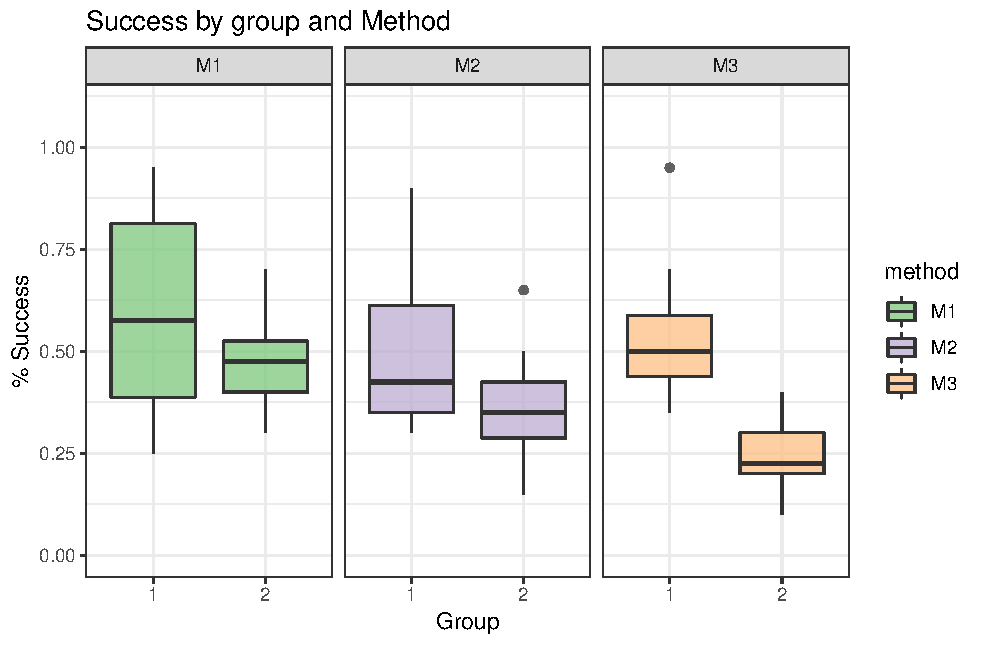
\includegraphics[scale=0.7]{plot1.pdf}
	\label{p1}
\end{figure}


\begin{enumerate}
	
	\item \textcolor{BlueGreen}{\textbf{Planteado con interacción}}
	\[X_{ijk}=\mu+\alpha_i+\beta_j+\gamma_{ij}+\epsilon_{ijk} ,\,\, \text{con} \,\, 1 \leq i \leq 3, 1 \leq j \leq 2 \,\, \text{con} \,\, 1 \leq k \leq 8
	\]
	siendo
	\[
	\epsilon_{ijk}\sim N(0,\sigma^2) \hspace{0.3cm} \text{independientes}
	\]
	\begin{itemize}
		\item $\alpha_i$ efecto del método i-esimo.
		\item $\beta_j$ efecto del j-esimo grupo.
	\end{itemize}
	\begin{itemize}
		\item $\alpha_i$ efecto del método i-esimo.
		\item $\beta_j$ efecto del j-esimo grupo.
		\item $\gamma_{ij}$ interacción entre el i-esimo método y el j-ésimo grupo.
	\end{itemize}

\begin{figure}[H]
	\centering
	\caption{Gráfico de Interacciones}
	\label{p4}
	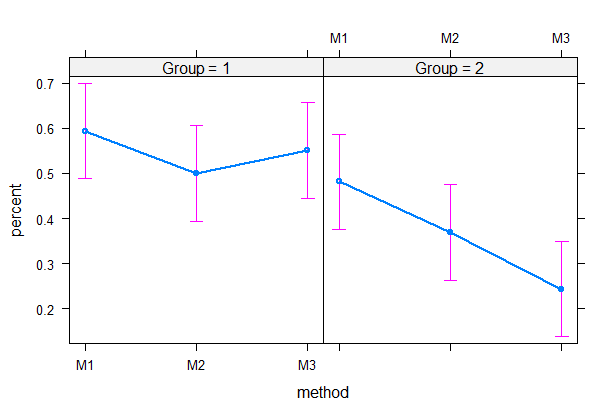
\includegraphics[scale=0.7]{plot4.png}
\end{figure}	

Analicemos la signficación del modelo.
\begin{table}[H]
	\centering
	\caption{Salida Anova Modelo con interacción}
	\begin{tabular}{lrrrrrr}
		& \multicolumn{1}{l}{Df} & \multicolumn{1}{l}{Sum Sq} & \multicolumn{1}{l}{Mean Sq} & \multicolumn{1}{l}{F value} & \multicolumn{1}{l}{P value} &  \\
		Group & 1     & 0.4033 & 0.4033 & 12.701 & 0.000 & \multicolumn{1}{l}{***} \\
		method & 2     & 0.1697 & 0.0848 & 2.672 & 0.080 & \multicolumn{1}{l}{.} \\
		Group:method & 2     & 0.0914 & 0.0457 & 1.438 & 0.248 &  \\
		Residuals & 42    & 1.3337 & 0.0318 &       &       &  \\
	\end{tabular}%
	\label{tab:anova1}%
\end{table}%

En esta salida se aprecia la no significación de la interacción, por lo cual en lo sucesivo trabajamos sin interacción.

	\item \textcolor{BlueGreen}{\textbf{Planteado sin interacción}}
	
	\[X_{ijk}=\mu+\alpha_i+\beta_j+\epsilon_{ijk} ,\,\, \text{con} \,\, 1 \leq i \leq 3, 1 \leq j \leq 2 \,\, \text{con} \,\, 1 \leq k \leq 8
	\]
	siendo
	\[
	\epsilon_{ijk}\sim N(0,\sigma^2) \hspace{0.3cm} \text{independientes}
	\]
	
\begin{table}[H]
	\centering
	\caption{Salida Anova Modelo sin interacción}
	\begin{tabular}{lrrrrrr}
		& \multicolumn{1}{l}{Df} & \multicolumn{1}{l}{Sum Sq} & \multicolumn{1}{l}{Mean Sq} & \multicolumn{1}{l}{F value} & \multicolumn{1}{l}{P value} &  \\
		Group & 1     & 0.4033 & 0.4033 & 12.45 & 0.000 & \multicolumn{1}{l}{***} \\
		method & 2     & 0.1697 & 0.0848 & 2.62  & 0.084 & \multicolumn{1}{l}{.} \\
		Residuals & 44    & 1.4251 & 0.0324 &       &       &  \\
	\end{tabular}%
	\label{anova2}%
\end{table}%

En la salida del modelo sin interacción, se aprecia que los porcentajes de acierto son significativamente diferentes en los dos grupos, pero no hay diferencias significativas entre los métodos de medición ensayados.	

	
\begin{table}[H]
	\centering
	\caption{Diferencias estimadas entre grupos }
	\begin{tabular}{rrrrr}
		\multicolumn{1}{l}{Group} &       &       &       &  \\
		& \multicolumn{1}{l}{diff} & \multicolumn{1}{l}{lwr} & \multicolumn{1}{l}{upr} & \multicolumn{1}{l}{p value} \\
		2-1 & 0.1833 & 0.07862 & 0.2880 & 0.000 \\
	\end{tabular}%
	\label{entregrupos}%
\end{table}%

	
	Como el intervalo de confianza no contiene al 0, la media de uno de los grupos es significativamente mayor que el otro.
	
	La diferencia estimada entre métodos es:	
	
	\begin{table}[H]
		\centering
		\caption{Diferencias estimadas entre métodos}
		\begin{tabular}{lrrrr}
			method &       &       &       &  \\
			& \multicolumn{1}{l}{diff} & \multicolumn{1}{l}{lwr} & \multicolumn{1}{l}{upr} & \multicolumn{1}{l}{p value} \\
			M2-M3 & 0.0375 & -0.11682& 0.1918 & 0.8265 \\
			M1-M3 & 0.140 & -0.01370 & 0.2949 & 0.0805 \\
			M1-M2 & 0.103 & -0.05120 & 0.2574 & 0.247 \\
		\end{tabular}%
		\label{entremetodos}%
	\end{table}%

\begin{figure}[H]
	\centering
	\caption{Intervalos de Confianza para diferencias entre Métodos}
	\label{plot3}
	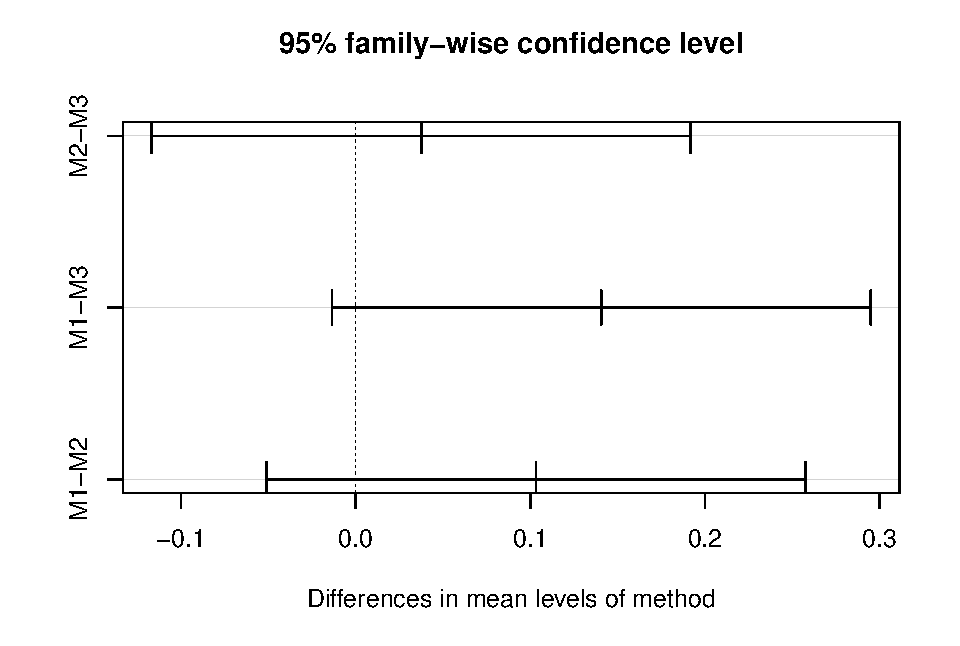
\includegraphics[scale=0.8]{plot3.pdf}
\end{figure}	

Todos los intervalos de confianza contienen el 0, por lo tanto no hay diferencias estadísticamente significativas por método.

\item \textcolor{BlueGreen}{\textbf{Planteado sin interacción con efecto aleatorio por individuo anidado en grupo}}
	\[X_{ijk}=\mu+\alpha_i+\beta_j+a_k(j)+\epsilon_{ijk} ,\,\, \text{con} \,\, 1 \leq i \leq 3, 1 \leq j \leq 2 \,\, \text{con} \,\, 1 \leq k \leq 8
	\]
	siendo $a_k(j)$ el efecto del k-simo individuo en el j-simo grupo.
	\[
	\epsilon_{ijk}\sim N(0,\sigma^2) \hspace{0.3cm} \text{independientes}
	\]
\end{enumerate}


\begin{table}[H]
	\centering
	\caption{Salida efectos fijos del modelo mixto}
	\begin{tabular}{lrrrrr}
		Fixed & \multicolumn{1}{l}{effects:} &       &       &       &  \\
		& \multicolumn{1}{l}{Value} & \multicolumn{1}{l}{Std.Error} & \multicolumn{1}{l}{DF} & \multicolumn{1}{l}{t-value} & \multicolumn{1}{l}{p-value} \\
		(Intercept) & 0.6292 & 0.0564 & 30.0000 & 11.1524 & 0 \\
		Group2 & -0.1833 & 0.0672 & 14.0000 & -2.7291 & 0.0163 \\
		methodM2 & -0.1031 & 0.0527 & 30.0000 & -1.9562 & 0.0598 \\
		methodM3 & -0.1406 & 0.0527 & 30.0000 & -2.6675 & 0.0122 \\
	\end{tabular}%
	\label{anova3}%
\end{table}%

Considerando a los individuos como un efecto aleatorio, aparecen significativas las disverencias entre grupos pero también aparece significativas las diferencias entre el tercer método de medición y el primero.

\subsubsection{Diagnóstico del Modelo}

En la Figura\ref{plot5} no se aprecia estructura en los residuos.
El test de Shapiro arroja un pvalor = 0.5396, lo cual permite sostener el supuesto de normalidad de los residuos del modelo.

\begin{figure}[H]
	\centering
	\caption{Residuos vs valores ajustados}
	\label{plot5}
	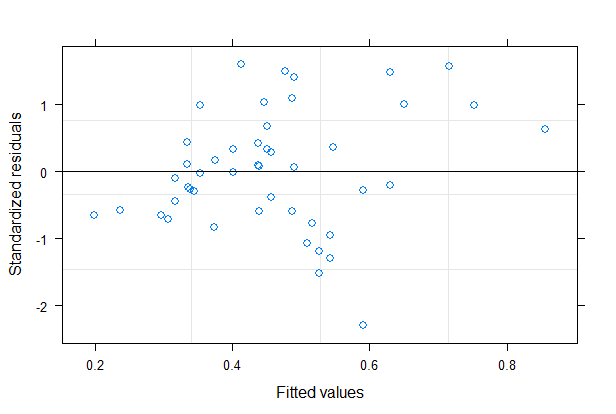
\includegraphics[scale=0.8]{plot5.png}
\end{figure}

En la Figura\ref{plot2} se comparan los cuantiles teóricos de una normal con los cuantiles empíricos de los residuos y se puede apreciar que los residuos se aproximan a una distribución normal.

\begin{figure}[H]
	\centering
	\caption{Qqplot de los residuos del modelo}
	\label{plot2}
	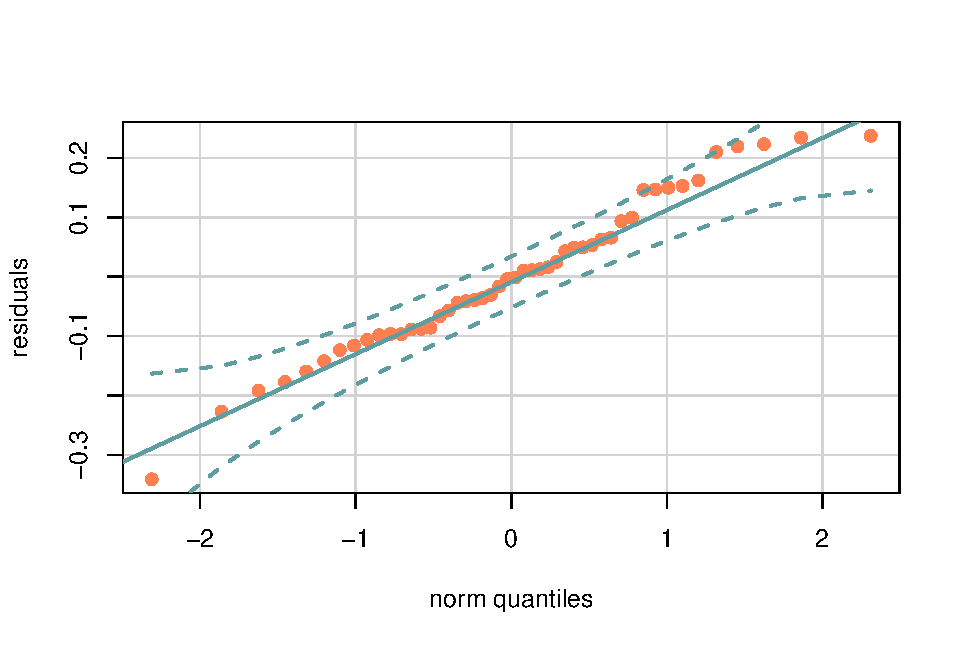
\includegraphics[scale=1]{plot2.pdf}
\end{figure}

Tampoco se rechaza el supuesto de homocedasticidad de los residuos. El p valor del test de Levenne es 0.85.
\end{document}